\documentclass{sigkddExp}

\usepackage[utf8]{inputenc}
\usepackage{mathptmx}
\usepackage{graphicx}
\usepackage{booktabs}
\usepackage{array}
\usepackage{xurl}

\pdfpagewidth=8.5in
\pdfpageheight=11in
\usepackage{etoolbox}
\makeatletter
\patchcmd{\@sect}{\vskip -14pt}{}{}{\errmessage{sigkddExp heading patch failed}}
\makeatother
\setcounter{secnumdepth}{2}
\renewcommand{\paragraph}[1]{\par\vspace{2pt}\noindent\textbf{#1.}\enskip}
\setlength{\tabcolsep}{3pt}
\sloppy
\hyphenation{Masakha-NER Afro-XLMR Mphaya-NER}
\let\oldthebibliography\thebibliography
\renewcommand{\thebibliography}[1]{\small\oldthebibliography{#1}\setlength{\itemsep}{0pt}\setlength{\parsep}{0pt}}

\newcommand{\ra}{$\rightarrow$}
\newcommand{\TR}{\mathrm{TR}}

\begin{document}

\title{Language, Domain, or Pretraining Exposure?\\
Cross-Lingual NER for South African Bantu Languages}
\numberofauthors{1}
\author{
\alignauthor Mpendulo Sibeko\\
\affaddr{Department of Computer Science, University of Pretoria}\\
\affaddr{Student number 19144832}\\
\email{u19144832@tuks.co.za}
}
\date{}
\maketitle

\section*{Abstract}
Zero-shot cross-lingual named entity recognition (NER) depends heavily on the choice of source language; however, it is not settled what makes a good source for South African Bantu languages. This study fine-tunes AfroXLMR-base on eleven sources from two corpora, NCHLT (government text) and MasakhaNER~2.0 (news), and evaluates each model on nine test sets in six languages, which gives 297 zero-shot and 36 few-shot evaluations over three seeds. Linguistic relatedness is the most consistent predictor of transfer ($+0.10$ transfer ratio per relatedness step, $p<.001$), and it remains significant when corpus terms and the tokenizer-fertility gap are added. However, corpus match can override relatedness: a sister-language news source beats a same-language government source by 32.0~F1 on isiZulu news and by 12.7~F1 on isiXhosa news (Holm $p=.005$), but not on isiXhosa or Setswana government text. Targets seen in AfroXLMR's pretraining do not transfer better than unseen targets, although exposure is confounded with language cluster. With 500 target sentences, 57--89\% of the gap to in-language performance closes. Contrary to our hypothesis, Swahili is a stronger Setswana source than Sepedi or Sesotho by 13.0--19.0~F1, and it stays ahead when every source is trained on the same number of entity spans. Since the two corpora differ in both text domain and annotation guidelines, we close by proposing experiments that could separate the two.

\smallskip
\noindent\textbf{Keywords:} cross-lingual transfer; named entity recognition; South African languages; low-resource NLP; AfroXLMR

\section{Introduction}\label{sec:intro}

Named entity recognition (NER) is the task of identifying people, places and organisations in text, and for South African Bantu languages it is held back by the small amount of labelled data. Cross-lingual transfer offers an alternative, where a multilingual encoder is fine-tuned on a better-resourced source language and then applied to the target language without any target training data. The choice of source has a large effect; for example, in MasakhaNER~2.0, David Ifeoluwa Adelani et al.~\cite{adelani2022} found that zero-shot isiXhosa F1 rose from 24.5 with an English source to 83.7 with an isiZulu source.

However, what makes a good source is less settled. Transfer has been linked to linguistic relatedness and pretraining exposure~\cite{devries2022,pires2019}, to token and entity overlap more than genetic distance~\cite{beukman2023,adelani2022}, and to factors whose value changes from one task to another~\cite{idris2026}. The evidence for South African languages is limited: MasakhaNER~2.0 covers news only and contains neither Sepedi nor Sesotho, which are Setswana's closest relatives~\cite{adelani2022}, and the only direct comparison of language and domain for NER that we found is a single Tshivenda result~\cite{mbuvha2023}.

Thus, this study asks: \emph{how are linguistic relatedness, domain match and documented pretraining exposure associated with zero-shot and few-shot NER transfer among six South African Bantu languages?} It answers the following research questions:
\begin{itemize}
  \item \textbf{RQ1.} Does linguistic relatedness or domain match better predict zero-shot transfer?
  \item \textbf{RQ2.} Do targets documented as seen in pretraining transfer better than unseen targets?
  \item \textbf{RQ3.} How far do 100 and 500 labelled target sentences close transfer gaps?
  \item \textbf{RQ4.} Are Sepedi and Sesotho stronger Setswana sources than Swahili and Chichewa, the top-ranked Setswana sources in MasakhaNER~2.0's LangRank analysis~\cite{lin2019,adelani2022}?
\end{itemize}
The hypotheses, as stated in the project proposal, are: \textbf{H1}, related sources transfer better on average, although domain match may reduce or reverse this; \textbf{H2}, seen targets show higher transfer ratios; \textbf{H3}, target data narrows transfer gaps; and \textbf{H4} (exploratory), Sepedi and Sesotho are better Setswana sources than Swahili and Chichewa, tested on Setswana news, where relatedness and domain conflict.

This study contributes to the pool of knowledge in four ways. First, it crosses source language with source corpus for NER among Nguni and Sotho-Tswana languages, with 333 evaluations of one model. Second, it tests Sepedi and Sesotho as Setswana sources, for which we found no transformer-based precedent. Third, it compares the few-shot curves of a related-language source with those of a same-language source from the other corpus. Fourth, it proposes follow-up experiments in Section~\ref{sec:future} that could separate text domain from annotation conventions.

The rest of this report is organised as follows: Section~\ref{sec:related} reviews related work, Sections~\ref{sec:data} and~\ref{sec:method} describe the data and method, Section~\ref{sec:results} presents the results and robustness checks, Section~\ref{sec:discussion} discusses them, and Sections~\ref{sec:limitations}--\ref{sec:conclusion} present the limitations, future work and conclusion.

\section{Related Work}\label{sec:related}

\subsection{Relatedness, overlap and domain (RQ1)}\label{sec:rw-rq1}
Telmo Pires et al.~\cite{pires2019} showed that multilingual encoders transfer NER between languages with almost no lexical overlap; however, overlap still predicts how much transfer occurs. For African NER, Michael Beukman and Manuel Fokam~\cite{beukman2023} found that token overlap correlates with transfer at Pearson $R=0.73$, against $-0.30$ for genetic distance, but their ten languages include no Southern Bantu language. In MasakhaNER~2.0, geographic distance and entity overlap were the most important features of the LangRank source ranker~\cite{lin2019}, and entity overlap correlated with transfer at Spearman $R=0.6$~\cite{adelani2022}. Furthermore, embedding similarity predicts NER transfer but only weakly predicts sentiment transfer~\cite{idris2026}, which means that no single predictor holds across tasks.

Studies that separate language shift from domain shift often find that domain costs as much as language. In DaN+, Barbara Plank et al.~\cite{plank2020} report that German\ra Danish news lost about 4~F1, while same-language shifts from news to social media lost about 13--40, and Maarten De Raedt et al.~\cite{deraedt2023} found for sentiment that domain-only drops are at least as large as language drops. In contrast, Antonio Martínez-García et al.~\cite{martinezgarcia2021} use correlational domain proxies and conclude that most transfer loss is not due to domain. The domain shifts in CrossNER also add entity types~\cite{liu2021crossner}, which ours do not. For South African languages, MphayaNER is the only direct contrast we found: Rendani Mbuvha et al.~\cite{mbuvha2023} report that every related-language news source beat Tshivenda government data on Tshivenda news (best 46.2 against 35.2), although from one target and without significance tests. Government-domain zero-shot transfer also appears to be hard, since NGLUEni reports 32.4 weighted F1 for isiXhosa\ra isiZulu on SADiLaR NER data~\cite{meyer2024}, against 82.1 entity F1 for the same pair on news in MasakhaNER~2.0, with a different model and metric~\cite{adelani2022}. Thus, no study crosses source language with source corpus for NER among South African Bantu languages, and in NCHLT versus MasakhaNER the domain coincides with the annotation guideline, which none of these studies separates.

\subsection{Datasets with different annotation conventions}\label{sec:rw-guidelines}
Training one model on datasets annotated under different conventions has precedents. Sara Stymne et al.~\cite{stymne2018} improved a multi-treebank dependency parser with a learned treebank embedding, by up to 3.5 LAS over single-treebank training and by over 2.0 over concatenation. Similarly, Gamal Crichton et al.~\cite{crichton2017} found that multi-task biomedical NER with dataset-specific outputs helped small datasets the most, and taggers have been trained over datasets whose tag sets only partly overlap~\cite{greenberg2018,huang2019}. Bottleneck adapters~\cite{houlsby2019,pfeiffer2020} give each dataset its own small set of parameters on a shared encoder. However, we found no study that separates annotation conventions from text domain in cross-corpus NER for these languages, and Section~\ref{sec:future} proposes how to do so.

\subsection{Pretraining exposure (RQ2)}\label{sec:rw-rq2}
Wietse de Vries et al.~\cite{devries2022} fitted a mixed-effects model of zero-shot POS transfer over more than 100 languages and found that target inclusion in pretraining was the strongest predictor, with an estimated 19.2\% higher accuracy. However, the gains from adaptation point the other way: in Glot500, languages unseen by XLM-R gain $+13.2$~F1 on WikiANN from inclusion, against $+2.1$ for head languages~\cite{imani2023}, and adaptation benefits unseen languages more than seen ones~\cite{ansell2022,faisal2022}. Furthermore, Phillip Rust et al.~\cite{rust2021} found that tokenizer quality matters about as much as the size of the pretraining data, therefore an exposure effect may partly be a tokenizer effect. AfroXLMR's adaptation corpus contains isiZulu, isiXhosa and Sesotho but not siSwati, Sepedi or Setswana~\cite{alabi2022}. In NGLUEni, AfroXLMR-large improved on XLM-R-large by $+2.1$ for seen isiZulu but by $+5.3$ and $+5.9$ for unseen isiNdebele and siSwati~\cite{meyer2024}. Thus, no study reports seen-versus-unseen NER transfer ratios for these languages, and every unseen target has a seen close relative.

\subsection{Few-shot target data (RQ3)}\label{sec:rw-rq3}
Anne Lauscher et al.~\cite{lauscher2020} fine-tuned XLM-R on English and then on $k$ target sentences, and it averaged 85.43 F1 on WikiANN at $k=0$, 91.49 at $k=100$ and 93.69 at $k=500$, which means that most of the gain arrives by 100 sentences. Mengjie Zhao et al.~\cite{zhao2021} found that the choice of sampled sentences causes more variance than the seed, and that plain fine-tuning beats more elaborate few-shot methods. In MasakhaNER~2.0, the best zero-shot source comes close to annotating 500 target sentences in most cases~\cite{adelani2022}. However, no study compares the learning curves of a related-language source and a same-language source from another domain for NER.

\subsection{Sources for Setswana (RQ4)}\label{sec:rw-rq4}
In MasakhaNER~2.0, Setswana's best single sources were German (73.3) and Swahili (73.1), LangRank's predicted top two were Swahili and Chichewa~\cite{lin2019}, and the pool had no Sotho-Tswana language~\cite{adelani2022}. The most direct evidence that Sotho-Tswana languages help each other comes from speech, where Christiaan Jacobs and Herman Kamper~\cite{jacobs2021} found that acoustic word embeddings for Sesotho trained on Sepedi and Setswana reached 76.7\% AP, against 51.9\% for isiXhosa and siSwati. PuoBERTa evaluates Setswana NER without cross-lingual experiments~\cite{marivate2023}, and the transfer study of Sindane uses static embeddings~\cite{sindane2023}. Thus, we found no transformer-based NER study that uses Sepedi or Sesotho as a source for Setswana.

\section{Data}\label{sec:data}

\paragraph{Corpora and languages} This study uses two public, human-annotated NER corpora with BIO tags (Table~\ref{tab:data}). NCHLT NER~\cite{eiselen2016} covers South African government text and has no official splits, therefore we shuffle each language once with a fixed seed and save one 80/10/10 train/dev/test split. MasakhaNER~2.0~\cite{adelani2022} covers news, and we keep its published splits. The six targets form two clusters: the Nguni languages isiZulu (zul), isiXhosa (xho) and siSwati (ssw), which are written conjunctively, and the Sotho-Tswana languages Sepedi (nso), Sesotho (sot) and Setswana (tsn), which are written disjunctively. Swahili (swa) and Chichewa (nya) are Bantu but not Southern Bantu languages, are written conjunctively, and serve only as sources. This gives nine test sets, six from NCHLT and three from MasakhaNER. isiZulu, isiXhosa and Setswana appear in both corpora, and these are the only cells in which language and corpus are fully crossed.

\begin{table}[t]
\centering\footnotesize
\caption{Corpora. NCHLT sizes are from our seeded 80/10/10 split after deduplication; MasakhaNER sizes are the downloaded splits before deduplication.}
\label{tab:data}
\begin{tabular}{@{}>{\raggedright}p{1.8cm}>{\raggedright}p{1.85cm}>{\raggedright\arraybackslash}p{4.15cm}@{}}
\toprule
Corpus & Languages & Size, labels, licence\\
\midrule
NCHLT NER (government) & zul, xho, ssw, nso, sot, tsn & $\geq$15,000 annotated entity tokens per language; train/dev/test: zul 8,680/1,085/1,086; xho 4,939/617/618; ssw 8,409/1,051/1,052; nso 5,584/698/698; sot 7,486/935/937; tsn 6,214/776/778; PER, LOC, ORG, MISC; CC BY 2.5 ZA\\
\addlinespace
MasakhaNER 2.0 (news) & zul, xho, tsn; swa, nya (sources only) & train/dev/test: zul 5,848/836/1,670; xho 5,718/817/1,633; tsn 3,489/499/996; train swa 6,593, nya 6,250; PER, LOC, ORG, DATE; CC BY-NC 4.0\\
\bottomrule
\end{tabular}
\end{table}

\paragraph{Label harmonisation and source cap} All experiments use the PER, LOC and ORG types. NCHLT \texttt{MISC} and MasakhaNER \texttt{DATE} spans, which make up 4--11\% of NCHLT tokens, are masked, meaning that they are excluded from the loss and from scoring instead of being relabelled as non-entities. Each source is capped at 3,000 training sentences, resampled with each seed. However, the cap equalises sentences and not entities: the estimated number of PER/LOC/ORG spans per 3,000 sentences ranges from about 5,600 (Swahili) to 1,900 (NCHLT Setswana), and Section~\ref{sec:res-robust} tests whether this matters.

\paragraph{Deduplication} The first complete run (v1) contained duplicate sentences that leaked between training and test data. We detected them by exact match on lower-cased, whitespace-normalised token sequences and removed 922 NCHLT sentences (0.9--2.6\% per language) and 626 MasakhaNER training and development sentences (at most 8.2\%, for the isiXhosa training data), while the MasakhaNER test sets keep their published sizes. All results come from the deduplicated run (v2). Removing the leakage lowered the most affected in-language scores (MasakhaNER isiXhosa 89.5\ra 88.1; NCHLT Setswana 81.6\ra 78.6), but it did not change the direction of any finding.

\paragraph{Exposure and tokenizer fertility} Following AfroXLMR's adaptation corpus~\cite{alabi2022}, isiZulu, isiXhosa and Sesotho are treated as \emph{seen} targets and siSwati, Sepedi and Setswana as \emph{unseen} targets. Tokenizer fertility, the number of subwords per word on the training data, is 1.51 for Swahili, 1.77--1.87 for the Sotho-Tswana corpora, 2.25 for Chichewa and 2.43--2.78 for the Nguni corpora (Figure~\ref{fig:fertility}). Furthermore, the NCHLT Sesotho corpus is anomalous: its in-language score is 59.5 here and 55.6 in SERENGETI~\cite{adebara2023}, against about 77--81 for Setswana and Sepedi~\cite{adebara2023,hanslo2022}.

\begin{figure}[t]
\centering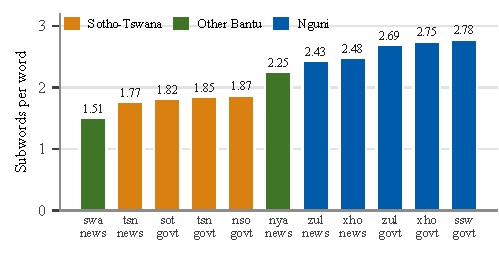
\includegraphics[width=\columnwidth]{figures/fertility_by_corpus}
\caption{AfroXLMR tokenizer fertility (subwords per word) on each training corpus, coloured by language group. Swahili's fertility is closer to that of the Sotho-Tswana corpora than Chichewa's or the Nguni corpora's.}
\label{fig:fertility}
\end{figure}

\section{Method}\label{sec:method}

\paragraph{Model and fine-tuning} All experiments use AfroXLMR-base (\texttt{Davlan/afro-xlmr-base}), which is an XLM-R-base model adapted to African languages~\cite{alabi2022}, with a linear token-classification head. A single set of hyperparameters is used for every comparison: AdamW, a learning rate of $5\times10^{-5}$, weight decay of 0.01, batch size 16, 3 epochs, linear decay with no warm-up, gradient clipping at 1.0, fp16 and a maximum length of 128 subword tokens. Every configuration is trained with seeds 13, 42 and 2026 and the final model is used, therefore no checkpoint is selected on development or target data.

\paragraph{Zero-shot grid} Eleven sources, namely the six NCHLT languages, the three MasakhaNER target languages, and MasakhaNER Swahili and Chichewa, are trained with three seeds and evaluated on all nine test sets, which gives 297 zero-shot evaluations. The nine pairs that share language and corpus give in-language upper bounds, and the other 90 are transfer pairs. Each transfer pair is coded for \emph{relatedness} on four ordinal levels (same language in the other corpus, same cluster, other Southern Bantu and other Bantu, where higher means closer), \emph{domain match} (same corpus), \emph{target exposure} (seen or unseen), source--target \emph{entity overlap} and, in exploratory models, the \emph{fertility gap}, which is the absolute difference in fertility. Since each corpus has its own guideline, domain match bundles text domain with annotation conventions.

\paragraph{Few-shot transfer} For each news target (isiZulu, isiXhosa and Setswana), two zero-shot models are fine-tuned further on $k\in\{100,500\}$ target sentences, resampled with each seed: the sister-language news source (isiXhosa for isiZulu and vice versa) and the same-language government source. No Sotho-Tswana news data exists, so Setswana's sister source is NCHLT Sepedi. This gives 36 evaluations, or 333 in total, with 10 epochs at $k=100$ and 5 at $k=500$.

\paragraph{Measures} The primary measure is entity-level micro-F1 with exact span match on PER, LOC and ORG. The \emph{transfer ratio} is $\TR(s\!\rightarrow\!t)=F1(s\!\rightarrow\!t)/F1(t\!\rightarrow\!t)$, which normalises for target difficulty. For few-shot runs, the \emph{gap closure} at $k$ is $(F1_k-F1_0)/(F1_{\mathrm{in}}-F1_0)$ and the \emph{share of gain by 100} is $(F1_{100}-F1_0)/(F1_{500}-F1_0)$. All scores are means over three seeds, and the seed standard deviations are mostly under 3~F1 (up to 6 for NCHLT Sesotho).

\paragraph{Statistics} Five contrasts were pre-specified. For RQ1, the sister-language news source is compared with the same-language government source on isiZulu news and on isiXhosa news; for RQ4, Sepedi and Sesotho are compared with Swahili on Setswana news, and Sepedi with Swahili on Setswana government text. Each contrast is a paired bootstrap over test sentences with 1,000 resamples~\cite{dror2018}, where every resample draws the same sentences for all three seeds and compares seed-averaged F1. Tests are one-sided in the hypothesised direction with Holm correction over the five contrasts, and two-sided values are also reported. With 1,000 resamples the smallest attainable one-sided $p$ is .001 (two-sided .002), therefore the Holm values of .005 and .01 reported below are at that floor. Moreover, the bootstrap resamples test sentences and not training runs, so it does not capture the training variance between seeds.

A linear mixed-effects regression (M0) of transfer ratio on relatedness, domain match, their interaction, exposure and entity overlap is fitted on the 90 seed-averaged transfer pairs with a random intercept for the target language; the proposal also specified a random intercept for the source language, which the fitted model omits. RQ3 is answered descriptively, and Table~\ref{tab:rqmap} maps each question to its test. The robustness checks in Section~\ref{sec:res-robust} were added after the main results and are not part of the Holm family.

\begin{table}[t]
\centering\footnotesize
\caption{How each research question is answered.}
\label{tab:rqmap}
\begin{tabular}{@{}l>{\raggedright}p{3.7cm}>{\raggedright\arraybackslash}p{2.6cm}@{}}
\toprule
RQ & Comparison & Measure and test\\
\midrule
RQ1 & Relatedness and domain match over 90 transfer pairs; sister-language news vs same-language government source on news targets & F1, TR; 2 bootstrap contrasts; M0\\
RQ2 & Seen (zul, xho, sot) vs unseen (ssw, nso, tsn) targets & F1, TR; exposure term in M0\\
RQ3 & 2 sources $\times$ 3 news targets, $k=0,100,500$ & F1, gap closure\\
RQ4 & Sepedi, Sesotho vs Swahili, Chichewa on both Setswana tests & F1; 3 bootstrap contrasts\\
\bottomrule
\end{tabular}
\end{table}

\section{Results}\label{sec:results}

Table~\ref{tab:verdicts} summarises the verdicts. Sections~\ref{sec:res-rq1}--\ref{sec:res-rq4} report the pre-specified analyses, and Section~\ref{sec:res-robust} reports the robustness checks that were added after the main results.

\begin{table*}[t]
\centering\footnotesize
\caption{Hypotheses and verdicts. Evidence marked $\dagger$ comes from post hoc robustness checks (Section~\ref{sec:res-robust}).}
\label{tab:verdicts}
\begin{tabular}{@{}l>{\raggedright}p{3.2cm}>{\raggedright\arraybackslash}p{12.6cm}@{}}
\toprule
Hyp. & Verdict & Key evidence\\
\midrule
H1 & Supported, with exceptions & Relatedness $+0.10$ TR per step ($p<.001$), also with corpus terms and the fertility gap$^\dagger$. A sister-language source from the target's corpus beats the same language from the other corpus on isiZulu news ($+32.0$~F1) and isiXhosa news ($+12.7$; both Holm $p=.005$), and on isiZulu government text ($+8.2$, not tested), but not on isiXhosa or Setswana government text\\
H2 & Not supported & Seen targets have neither higher F1 nor higher TR, and exposure is not significant ($p=.19$--$.36$). Exposure is confounded with cluster and fertility, so the result is inconclusive and not negative\\
H3 & Supported & 500 target sentences close 57--89\% of every gap. Most of the gain arrives by 100 sentences only for the two weakest starting points\\
H4 & Rejected (reversed) & Swahili beats Sepedi and Sesotho on Setswana news by 14.3 and 19.0~F1, and Sepedi on Setswana government text by 13.0 (two-sided Holm $p=.01$). The gap is unchanged with equal entity counts$^\dagger$\\
\bottomrule
\end{tabular}
\end{table*}

\subsection{RQ1: Relatedness versus domain match}\label{sec:res-rq1}
Relatedness is the most consistent predictor of zero-shot transfer (Figures~\ref{fig:heatmap} and~\ref{fig:rq1}). Same-language and same-cluster sources average 56--61~F1, against 37--47 for sources from other clusters, and at every relatedness level a source from the test set's own corpus adds only 0.04--0.08 to the transfer ratio. In M0, relatedness adds $+0.10$ to the transfer ratio per step ($p<.001$, 95\% CI 0.05--0.15), whereas neither the domain-match term ($p=.71$) nor its interaction with relatedness ($p=.79$) is significant.

In contrast, the pre-specified contrasts show where corpus match overrides relatedness (Table~\ref{tab:rq1}). On both news targets, a sister-language news source beats a same-language government source, by 32.0~F1 for isiZulu and by 12.7 for isiXhosa (both Holm $p=.005$, and positive in every seed). On government targets the picture is mixed: the sister-language government source also wins for isiZulu ($+8.2$), but the same-language news source wins for isiXhosa ($+21.4$) and Setswana ($+5.6$ to $+13.4$). Furthermore, transfer inside NCHLT is uneven, since isiZulu and isiXhosa reach only 46--52~F1 on each other's NCHLT test sets, against about 83 on news, where our sister-pair results match MasakhaNER~2.0 (82.4 vs 82.1; 82.7 vs 83.7, with a different model)~\cite{adelani2022}.

\begin{figure}[t]
\centering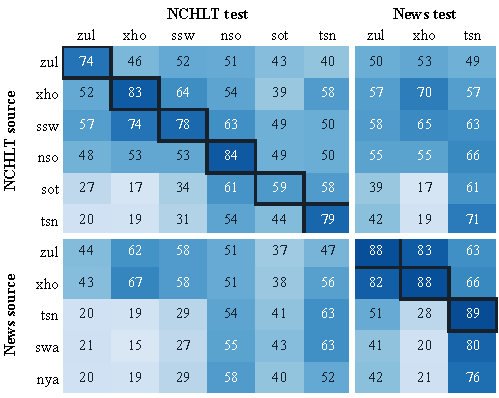
\includegraphics[width=\columnwidth]{figures/zero_shot_heatmap}
\caption{Zero-shot F1 for all source--test pairs (mean of 3 seeds, rounded). Rows are sources and columns are test sets; in-language cells are outlined.}
\label{fig:heatmap}
\end{figure}

\begin{figure}[t]
\centering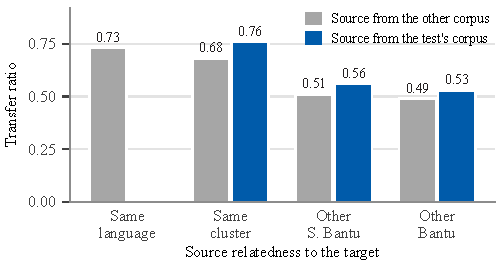
\includegraphics[width=\columnwidth]{figures/rq1_relatedness_corpus}
\caption{RQ1: mean transfer ratio by source relatedness and by whether the source comes from the test set's corpus (seed-level transfer pairs). A same-language source is always from the other corpus.}
\label{fig:rq1}
\end{figure}

\begin{table}[t]
\centering\footnotesize
\caption{RQ1: sister language in the same corpus vs same language in the other corpus (F1, mean of 3 seeds). $^*$Pre-specified, Holm $p=.005$.}
\label{tab:rq1}
\begin{tabular}{@{}lllr@{}}
\toprule
Test & Sister, same corpus & Same lang., other & $\Delta$\\
\midrule
zul news & xho news 82.4 & zul govt 50.4 & $+32.0^*$\\
xho news & zul news 82.7 & xho govt 70.0 & $+12.7^*$\\
zul govt & xho govt 52.4 & zul news 44.2 & $+8.2$\\
xho govt & zul govt 45.9 & xho news 67.3 & $-21.4$\\
tsn govt & nso govt 49.9 & tsn news 63.3 & $-13.4$\\
tsn govt & sot govt 57.7 & tsn news 63.3 & $-5.6$\\
\bottomrule
\end{tabular}
\end{table}

\paragraph{H1 verdict} Supported, with exceptions. Relatedness is the stronger general predictor; however, matching the target's corpus overrides it in three of the six comparisons, including both pre-specified news contrasts. Since each corpus has its own annotation guideline, this ``domain'' effect may come from the text, the labels or both.

\subsection{RQ2: Pretraining exposure}\label{sec:res-rq2}
Unseen targets score as high as or higher than seen targets at every relatedness level (Table~\ref{tab:rq2}), and the in-language NCHLT scores are highest for unseen Sepedi (83.6) and lowest for seen Sesotho (59.5). Exposure is not significant in any regression ($p=.19$--$.36$). In fact, from distant (other-Bantu) sources the transfer ratio is higher for unseen targets (0.66 against 0.38). However, two of the three unseen targets are Sotho-Tswana languages, which accept low-fertility sources such as Swahili well; therefore, exposure, cluster and fertility move together, and the anomalous Sesotho corpus lowers the seen group.

\begin{table}[t]
\centering\footnotesize
\caption{RQ2: mean zero-shot F1 by source relatedness and target exposure. The unseen same-language cell has one language (Setswana).}
\label{tab:rq2}
\begin{tabular}{@{}lrr@{}}
\toprule
Source relatedness & Seen targets & Unseen targets\\
\midrule
Same language (other corpus) & 58.0 & 67.0\\
Same cluster & 57.7 & 57.8\\
Other Southern Bantu & 35.1 & 50.8\\
Other Bantu & 28.2 & 55.1\\
\bottomrule
\end{tabular}
\end{table}

\paragraph{H2 verdict} Not supported. With six targets, exposure cannot be separated from cluster, fertility and corpus quality, so the absence of an advantage is inconclusive and not evidence against exposure.

\subsection{RQ3: Few-shot target data}\label{sec:res-rq3}
With 500 target sentences every gap narrows (Figure~\ref{fig:rq3}, Table~\ref{tab:rq3}), and 57--89\% of the gap to the in-language model closes. Government sources nearly catch up with sister-language news sources (isiZulu 83.5 vs 86.2; isiXhosa 83.6 vs 85.8), and for Setswana the Sepedi source (85.1) slightly passes the Setswana government source (84.0). The shape of the curves differs from the common finding that most of the gain arrives by 100 sentences~\cite{lauscher2020}. This holds only for the two sources furthest from the target (75\% and 62\%), whereas near-ceiling sources gain mainly between 100 and 500 sentences, and the isiZulu news source for isiXhosa does not improve at all by 100 sentences. For those sources the total gain is only 3--4~F1, which is close to seed variation, so their shares are imprecise.

\begin{figure*}[t]
\centering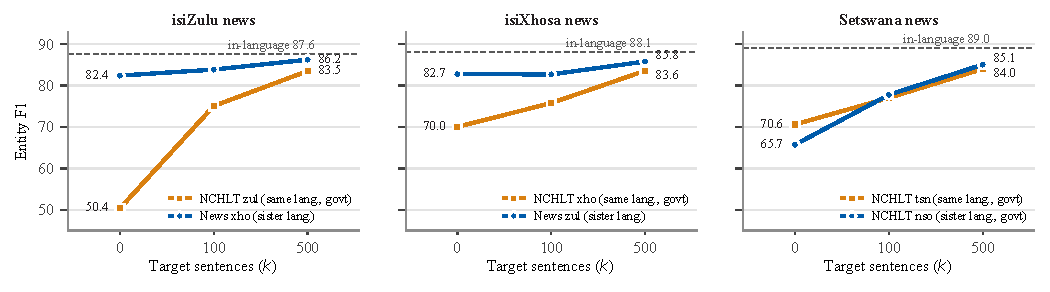
\includegraphics[width=\textwidth]{figures/rq3_fewshot_curves}
\caption{RQ3: few-shot learning curves on the three news targets (mean of 3 seeds). Orange: the same language from the government corpus; blue: a sister language. The dashed line is the in-language model.}
\label{fig:rq3}
\end{figure*}

\begin{table}[t]
\centering\footnotesize
\caption{RQ3: few-shot F1 (mean of 3 seeds) and share of the 500-sentence gain reached by $k=100$.}
\label{tab:rq3}
\begin{tabular}{@{}lrrrr@{}}
\toprule
Source \ra\ target & $k=0$ & $k=100$ & $k=500$ & By 100\\
\midrule
NCHLT zul \ra\ zul news & 50.4 & 75.1 & 83.5 & 75\%\\
NCHLT nso \ra\ tsn news & 65.7 & 77.8 & 85.1 & 62\%\\
NCHLT tsn \ra\ tsn news & 70.6 & 77.0 & 84.0 & 48\%\\
NCHLT xho \ra\ xho news & 70.0 & 75.8 & 83.6 & 42\%\\
News xho \ra\ zul news & 82.4 & 83.9 & 86.2 & 38\%\\
News zul \ra\ xho news & 82.7 & 82.7 & 85.8 & $-2$\%\\
\bottomrule
\end{tabular}
\end{table}

\paragraph{H3 verdict} Supported. 500 target sentences narrow every transfer gap, and they do so most quickly for weak, cross-corpus starting points.

\subsection{RQ4: Sources for Setswana}\label{sec:res-rq4}
H4 is rejected (Figure~\ref{fig:rq4}, Table~\ref{tab:rq4}). On Setswana news, Swahili (80.0) outperforms Sepedi (65.7) and Sesotho (61.0) in all three pre-specified contrasts, by 13.0--19.0~F1 and in every seed, and Chichewa (76.3) also scores above both, although no Chichewa contrast was pre-specified. The one-sided tests in the hypothesised direction give $p=1.0$, while the two-sided Holm $p$ is .01 for each contrast. Swahili is also the best other-language source on the Setswana government test (62.9). Since every Sotho-Tswana source is government text and every distant-Bantu source is news, the comparison confounds relatedness with corpus. Within NCHLT, where the corpus is fixed, Sepedi (49.9) and Sesotho (57.7) are no better than isiXhosa (57.7) on Setswana. Swahili lands well above the best published single-source scores for Setswana (73.1--73.3, with a different model and setting)~\cite{adelani2022}, and Sepedi lands below them.

\begin{figure*}[t]
\centering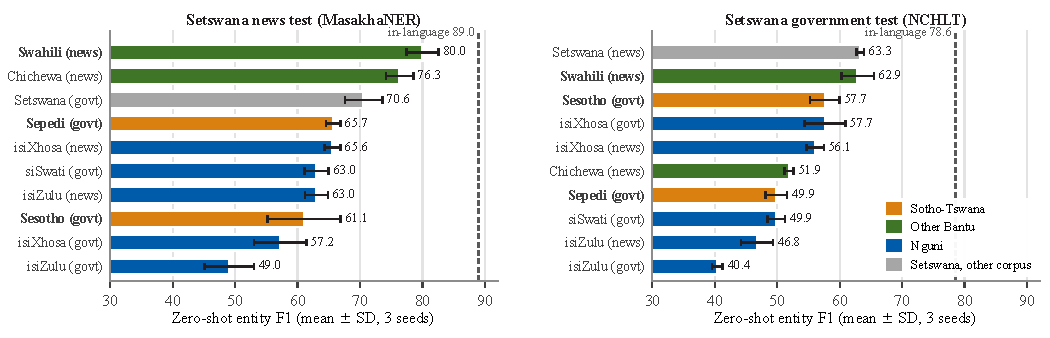
\includegraphics[width=\textwidth]{figures/rq4_setswana_sources}
\caption{RQ4: zero-shot F1 of every source on the two Setswana test sets (mean $\pm$ SD over 3 seeds), coloured by the source's language group. The three pre-specified sources are in bold; the dashed line is the in-language model.}
\label{fig:rq4}
\end{figure*}

\begin{table}[t]
\centering\footnotesize
\caption{RQ4: F1 on the two Setswana test sets with the 3,000-sentence cap and ($\dagger$, post hoc, Section~\ref{sec:res-robust}) with every source capped at 2,500 entity spans.}
\label{tab:rq4}
\begin{tabular}{@{}lrrrr@{}}
\toprule
& \multicolumn{2}{c}{News test} & \multicolumn{2}{c}{Govt test}\\
\cmidrule(lr){2-3}\cmidrule(l){4-5}
Source & sent.\ cap & ent.\ cap$^\dagger$ & sent.\ cap & ent.\ cap$^\dagger$\\
\midrule
Swahili (news) & \textbf{80.0} & 78.5 & 62.9 & 61.2\\
Chichewa (news) & 76.3 & 73.2 & 51.9 & 49.0\\
Sepedi (govt) & 65.7 & 64.2 & 49.9 & 48.7\\
Sesotho (govt) & 61.0 & 61.4 & 57.7 & 54.6\\
isiXhosa (govt) & 57.2 & 60.5 & 57.7 & 58.1\\
Setswana, other corpus & 70.6 & -- & \textbf{63.3} & --\\
\midrule
Setswana, in-language & 89.0 & -- & 78.6 & --\\
\bottomrule
\end{tabular}
\end{table}

\paragraph{H4 verdict} Rejected. On Setswana news, Swahili is a stronger source than Sepedi and Sesotho, and Chichewa also scores above both.

\subsection{Robustness checks}\label{sec:res-robust}
These checks were added after the main results and are not part of the Holm family.

\paragraph{Entity density and truncation} We re-trained the RQ4 sources on about 2,500 PER/LOC/ORG spans each (3 seeds; Table~\ref{tab:rq4}). The Swahili--Sepedi gap on Setswana news stays at 14.3~F1 (12.5 on government text), although Swahili reaches it from about half as many sentences (about 1,360 against 2,470). Furthermore, at 128 subword tokens at most 2.8\% of gold entities are truncated (NCHLT Setswana), and none are truncated in the news test sets.

\paragraph{Corpus terms and fertility} Replacing domain match in M0 with a source-corpus term and its interaction with the test corpus (M1) shows that a news source does not help government targets ($+0.016$, $p=.70$), but adds about 0.11--0.14 TR on news targets ($p=.12$; $p=.049$ once the fertility gap is added in M2). The fertility gap, which is the absolute difference in subwords per word between source and target, is the strongest added predictor ($-0.177$ TR per unit, $p=.001$; AIC $-71.2\rightarrow-78.8$), and it absorbs about a third of the relatedness coefficient ($0.112\rightarrow0.078$), which stays significant. Fertility and cluster are partly collinear; however, fertility fits an asymmetry that orthography does not. Swahili and Chichewa are written conjunctively like the Nguni languages, yet they transfer well to Sotho-Tswana targets, and Swahili's fertility (1.51) is close to that of the Sotho-Tswana corpora (about 1.8). Since the models have no source random intercept, the $p$-values of these source-level terms are likely optimistic.

\section{Discussion}\label{sec:discussion}

\paragraph{Relatedness and tokenizer fit} Relatedness is the most consistent predictor of transfer in this design, and about a third of its effect is shared with the tokenizer-fertility gap. Fertility helps to explain pairs that relatedness alone does not, such as Swahili transferring well into the Sotho-Tswana languages. However, the two are partly collinear here, therefore we treat fertility as a candidate mechanism behind part of the relatedness effect and not as a replacement for it.

\paragraph{What ``domain match'' measures} The corpus effect is concentrated in isiZulu and in news targets: a same-corpus sister language beats the same language from the other corpus by 32.0~F1 on isiZulu news, while on isiXhosa and Setswana government text the same-language news source wins. NCHLT and MasakhaNER differ in text domain, but they also differ in annotation guidelines and annotation teams. Thus, our design cannot tell whether the corpus effect comes from the text or from how each corpus defines an entity, for example whether titles and role words belong inside person spans. This distinction matters in practice because labelling conventions can be changed while domain cannot, and Section~\ref{sec:future} proposes experiments that separate the two.

\paragraph{Exposure and the Setswana reversal} Documented pretraining exposure showed no detectable association; however, with three seen and three unseen targets that line up with the language clusters, the design has little power to find one. For Setswana, Swahili outperforms both Sotho-Tswana relatives, and an equal number of entity spans does not change this. Since the relatives come only from government text and Swahili comes from news, the reversal is again an effect of source language and corpus together.

\paragraph{Relation to prior work} The advantage of news sources over government sources agrees with MphayaNER, where related-language news sources beat Tshivenda government data~\cite{mbuvha2023}, and with the low government-domain zero-shot scores in NGLUEni~\cite{meyer2024}. Furthermore, our Setswana ranking extends the MasakhaNER~2.0 LangRank analysis~\cite{lin2019,adelani2022} with the two Sotho-Tswana relatives that it could not include, and as annotated, both rank below Swahili.

\paragraph{Practical implications} For news NER in these languages, a news-annotated related source is a better starting point than same-language government data, and Swahili is a strong Setswana source. One hundred target sentences help the most when the only available source comes from the other corpus, and 500 sentences bring every source to within 1--5~F1 of the in-language model.

\section{Limitations}\label{sec:limitations}
This study is limited to one model (AfroXLMR-base) and three seeds. The bootstrap captures the variance of the test sample and not the training variance, and the regressions have a random intercept for the six target languages only, although the proposal also specified one for the source language. Furthermore, M0 converged at the boundary of the parameter space.

Domain match is corpus match, which means that it bundles text domain, annotation guideline and annotation team, therefore all effects are associations. Same-language pairs are always cross-corpus, and the two other-Bantu sources are always news. Moreover, RQ2 has only six targets, which are confounded with cluster, fertility and the anomalous Sesotho corpus, and in RQ4 the source language and source corpus coincide.

The pre-specified RQ4 tests were one-sided in the hypothesised direction and gave $p=1.0$; therefore, the significance of the reversal rests on two-sided tests, which we read as a post hoc result. Similarly, the robustness checks in Section~\ref{sec:res-robust} were designed after seeing the main results.

\section{Future Work}\label{sec:future}
The main open question is whether the corpus effect in RQ1 and RQ4 comes from the text domain or from annotation conventions. We ran preliminary versions of steps (1)--(3) after seeing the main results; however, they were designed post hoc and are not yet validated, therefore we do not report them here.
(1)~\textit{Error analysis:} every cross-corpus error is classified as a missed entity, a boundary error, a type error or a spurious prediction, and strict matching is compared with relaxed (overlap) matching and per-type F1, to see whether the gap reflects recognition failures or different definitions of an entity.
(2)~\textit{Guideline-specific heads:} one encoder is trained jointly on a language's two corpora with a separate adapter and output head for each guideline~\cite{stymne2018,crichton2017,houlsby2019,pfeiffer2020}. Scoring the same test text through each head then estimates how much of the cross-corpus gap the guideline alone accounts for.
(3)~\textit{Relabelling a related source:} titles, role nouns and generic institution nouns in the Sepedi and Sesotho training labels are rewritten towards news conventions, using a word list checked by at least two Setswana speakers per word, and the result is compared with a matched random-relabelling control. If a relabelled Sotho-Tswana source overtakes Swahili, the RQ4 reversal is a labelling effect.
(4)~\textit{A causal test:} two Setswana annotators relabel a blind sample of 200 test sentences from both corpora under one shared guideline (about 10--12 person-hours), and the cross-corpus gap is recomputed from the saved predictions.
(5)~\textit{Exposure and uncertainty:} an XLM-R-base contrast, which shares AfroXLMR's tokenizer but not its exposure, is the proper test for RQ2~\cite{conneau2020,alabi2022}. Moreover, more seeds, confidence intervals and crossed source and target random effects would tighten every estimate.

\section{Conclusion}\label{sec:conclusion}
This study asked how linguistic relatedness, domain match and documented pretraining exposure are associated with NER transfer among six South African Bantu languages. Relatedness is the most consistent predictor (RQ1), and it stays significant once corpus terms and the tokenizer-fertility gap are added; however, matching the target's corpus overrides it for isiZulu and for isiXhosa news. Targets seen in pretraining show no advantage (RQ2), although the design cannot separate exposure from cluster and fertility. Target data closes 57--89\% of transfer gaps with 500 sentences, and it does so fastest for weak cross-corpus sources (RQ3). For Setswana, Swahili is a stronger source than Sepedi or Sesotho, also with equal entity counts (RQ4).

Since the two corpora differ in both text and annotation guidelines, the corpus effects in RQ1 and RQ4 are associations whose cause remains open. Therefore, the most direct next question is whether a Sotho-Tswana source annotated consistently with the target would overtake Swahili, and the experiments in Section~\ref{sec:future} are designed to answer it.

\section*{Acknowledgements}
We thank the COS802 lecturers and the six reviewers who checked a Setswana word list for the planned relabelling study. The experiments were run on Google Colab.


\bibliographystyle{abbrv}
\bibliography{references}

\end{document}
